\documentclass[screen]{beamer}
\usepackage[T1]{fontenc}
\usepackage[utf8]{inputenc}
\usetheme{ntnubokmaal}
\usepackage{wasysym}
\usepackage{color}
\usepackage{allrunes}
\providecommand*{\wb}{{\textarl{\withlines futhark}}}

%Diverse matematiske lurerier
% \DeclareMathOperator{\Sample}{Sample}
\let\vaccent=\v % rename builtin command \v{} to \vaccent{}
\renewcommand{\v}[1]{\ensuremath{\mathbf{#1}}} % for vectors
\newcommand{\gv}[1]{\ensuremath{\mbox{\boldmath$ #1 $}}} 
% for vectors of Greek letters
\newcommand{\uv}[1]{\ensuremath{\mathbf{\hat{#1}}}} % for unit vector
\newcommand{\abs}[1]{\left| #1 \right|} % for absolute value
\newcommand{\avg}[1]{\left< #1 \right>} % for average
\let\underdot=\d % rename builtin command \d{} to \underdot{}
\renewcommand{\d}[2]{\frac{d #1}{d #2}} % for derivatives
\newcommand{\dd}[2]{\frac{d^2 #1}{d #2^2}} % for double derivatives
\newcommand{\pd}[2]{\frac{\partial #1}{\partial #2}} 
% for partial derivatives
\newcommand{\pdd}[2]{\frac{\partial^2 #1}{\partial #2^2}} 
% for double partial derivatives
\newcommand{\pdc}[3]{\left( \frac{\partial #1}{\partial #2}
 \right)_{#3}} % for thermodynamic partial derivatives
\newcommand{\ket}[1]{\left| #1 \right>} % for Dirac bras
\newcommand{\bra}[1]{\left< #1 \right|} % for Dirac kets
\newcommand{\braket}[2]{\left< #1 \vphantom{#2} \right|
 \left. #2 \vphantom{#1} \right>} % for Dirac brackets
\newcommand{\matrixel}[3]{\left< #1 \vphantom{#2#3} \right|
 #2 \left| #3 \vphantom{#1#2} \right>} % for Dirac matrix elements
\newcommand{\grad}[1]{\gv{\nabla} #1} % for gradient
\let\divsymb=\div % rename builtin command \div to \divsymb
\renewcommand{\div}[1]{\gv{\nabla} \cdot #1} % for divergence
\newcommand{\curl}[1]{\gv{\nabla} \times #1} % for curl
\let\baraccent=\= % rename builtin command \= to \baraccent


\title[Resultater \wb]{Resultater fra Futhark, MiA 2011}
\subtitle{Steking av bacon i mikrobølgeovn}
\author[Futhark]{Å. Ervik, K. H. Skrede, T. S. Solberg, P. Vo, J. Johnsen}
\institute[NTNU]{Eksperter i Team, NTNU}
\setbeamertemplate{footline}[ntnu theme nologo]
\date{13.04.2011}

\newcounter{saveenumi}
%\newcommand{\labelitemi}{$\bullet$}
\newcommand{\checktick}{\textcolor{green}{\checked}}

\begin{document}
\ntnutitlepage

\begin{frame}
  \frametitle{Motivasjon}
  \begin{center}
  \begin{figure}[!h]
    \begin{center}
      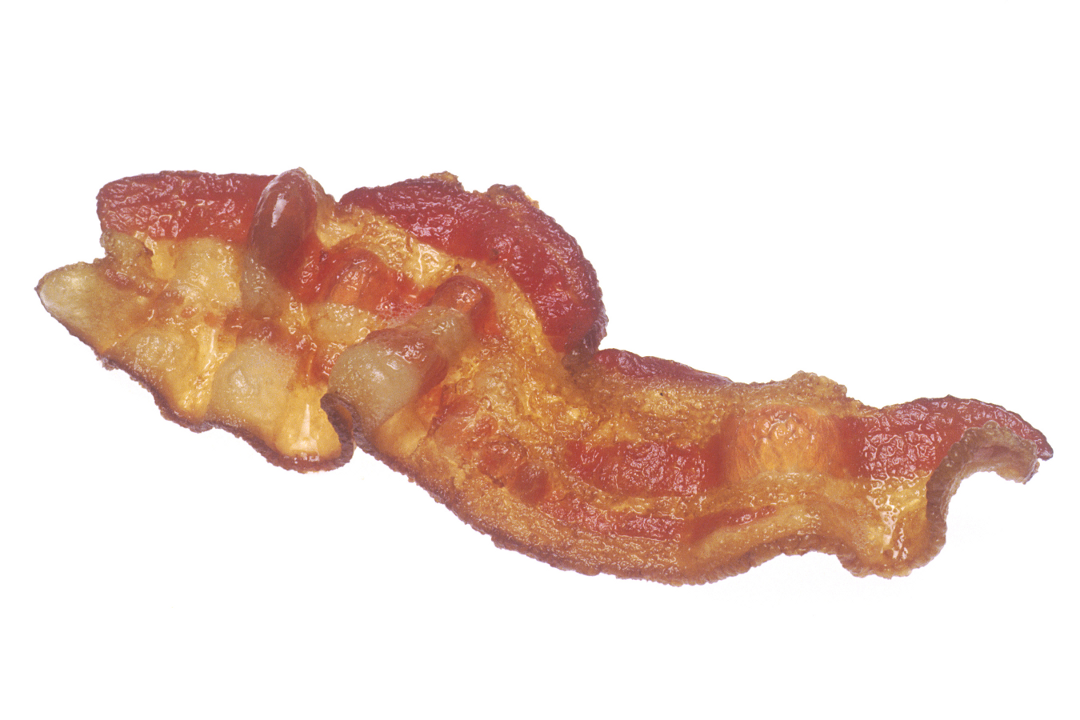
\includegraphics[width=0.6\textwidth]{bacon.png}
    \end{center}
    \caption{Mmmmm\ldots}
  \end{figure}
  \end{center}
\end{frame}

\begin{frame} 
  \frametitle{Problemstilling} 
  \begin{center} 
  \begin{itemize} 
  \item[$\bullet$] Hvordan kan steking av bacon i en mikrobølgeovn modelleres matematisk? 
  \item[$\bullet$] Hvordan vil fett og vanninnhold påvirke stekingen, og hvilken steketid er optimal? 
  \end{itemize} 
  \end{center} 
\end{frame}

\begin{frame}
  \frametitle{Planen}
  \begin{enumerate}
  \item Varme
  \item Massetransport
  \item Nøyaktige grensebetingelser for mikrobølgeovn
    \setcounter{saveenumi}{\theenumi}
\end{enumerate}
    \hline
\begin{enumerate}
    \setcounter{enumi}{\thesaveenumi}
  \item Elektromagnetiske grensebetingelser
  \item App - redusert modell
  \end{enumerate}
\end{frame}

\begin{frame}
  \frametitle{Planen}
  \begin{enumerate}
  \item[\checktick] Varme
  \item[2.] Massetransport
  \item[\checktick] Nøyaktige grensebetingelser for mikrobølgeovn
\end{enumerate}
    \hline
\begin{enumerate}
  \item[4.] Elektromagnetiske grensebetingelser
  \item[5.] App - redusert modell
  \end{enumerate}
\end{frame}

\begin{frame}
\frametitle{Difflikninger}
\begin{itemize}
  \item Varmelikninger
\end{itemize}
\begin{align*}
  \label{eq:temp}
  (\rho c_p)_m \pd{T}{t} &- \alpha_m \grad{^2 T} = J^{MW} \quad \rm{,} \\
  \eta_s (\rho c_p)_s \pd{T}{t} &- \eta_s\alpha_s \grad{^2 T} = J^{MW} - J^{Melt}  \quad \rm{,} \\
  \eta_l (\rho c_p)_l \pd{T}{t} &- \eta_s\alpha_l \grad{^2 T} - \eta_l(\rho c_p)_l(\v{v}\cdot
  \grad{})T = J^{MW}  \quad \rm{.}
\end{align*}
\begin{itemize}
  \item Massetransportlikning
\end{itemize}
\begin{equation*}
  \rho \left(\pd{v}{t} + v \cdot \pd{v}{x}\right) = -\pd{p}{x} + \mu \nabla^2 v + f
 \label{eq:navier-stokes}
\end{equation*}
\end{frame}

\begin{frame}
  \frametitle{Numerisk løsningsmodell}
  \begin{itemize}
    \item[$\bullet$] Vi bruker Finite Difference Method (FDM) til å løse differensial-
ligningene presentert i forrige slide.

\item[$\bullet$] Vi bruker et vanlig grid. For å sikre stabilitet har vi valgt
å bruke Crank-Nicolson:

\begin{eqnarray*}
u_m^{n+1}-\mu k(\frac{1}{h^2}\delta_x^2 u_m^{n+1}-\frac{1}{f^2}\delta_y^2 u_m^{n+1}-\frac{1}{g^2}\delta_z^2 u_m^{n+1})= &  \\
u_m^n + \mu k(\frac{1}{h^2}\delta_x^2 u_m^n + \frac{1}{f^2}\delta_y^2 u_m^n +\frac{1}{g^2}\delta_z^2 u_m^n)&
\end{eqnarray*}
der
\begin{equation*}
\delta_{r}^{2}U_m^{n}=\frac{U_{m+1}^{n}-2U_m^{n}+U_{m-1}^{n}}{{\Delta r}^{2}} \rm{,} \quad \quad \mu =\frac{\eta\alpha}{(\rho c_p)}
\end{equation*}


  \end{itemize}
\end{frame}

\begin{frame}
  \frametitle{Løsningskriterier}
  \begin{center}
  \begin{itemize}  
    \item[$\bullet$] \textbf{Q:} Hva får vår numeriske modell
      til å avslutte simuleringen?

    \item[$\bullet$] \textbf{Massedifferanse:} Baconpakning gir fettinnholdet ved start,
  massetransportligninger gjør det mulig å finne kritisk massetap (målt gjennom forsøk).

\item[$\bullet$] \textbf{Temperatur:} Maillards reaksjoner sier at bruning starter ved
  154$^o$C. Kritisk temperatur.
  \end{itemize}
  \end{center}
\end{frame}

\begin{frame}
  \frametitle{Status eksperimenter}
    \begin{center}
      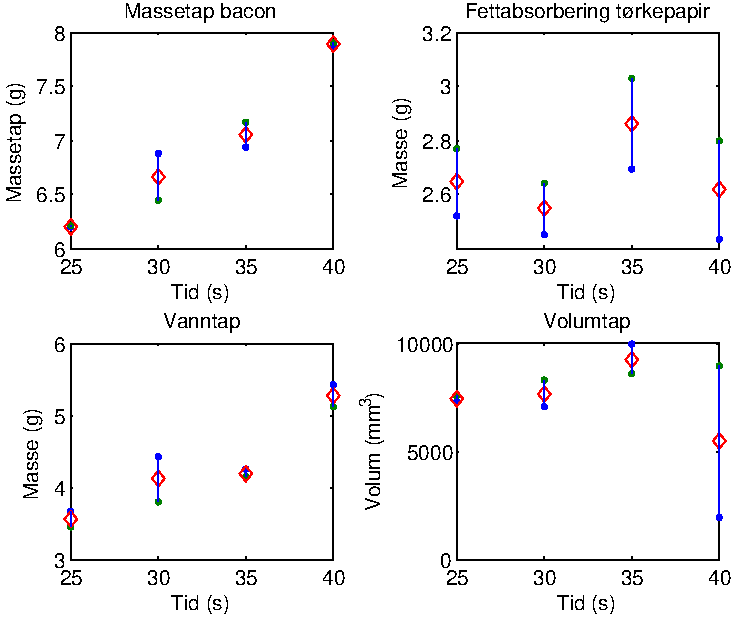
\includegraphics[width=0.7\linewidth]{eksperiment.pdf}
    \end{center}
\end{frame}

\begin{frame}
  \frametitle{Konklusjon}
  \begin{itemize}
    \item 
  \end{itemize}
\end{frame}

\end{document}



